\section*{}
\addcontentsline{toc}{section}{\scshape\large Discours sur le dessein de cette logique}

\begin{center}
	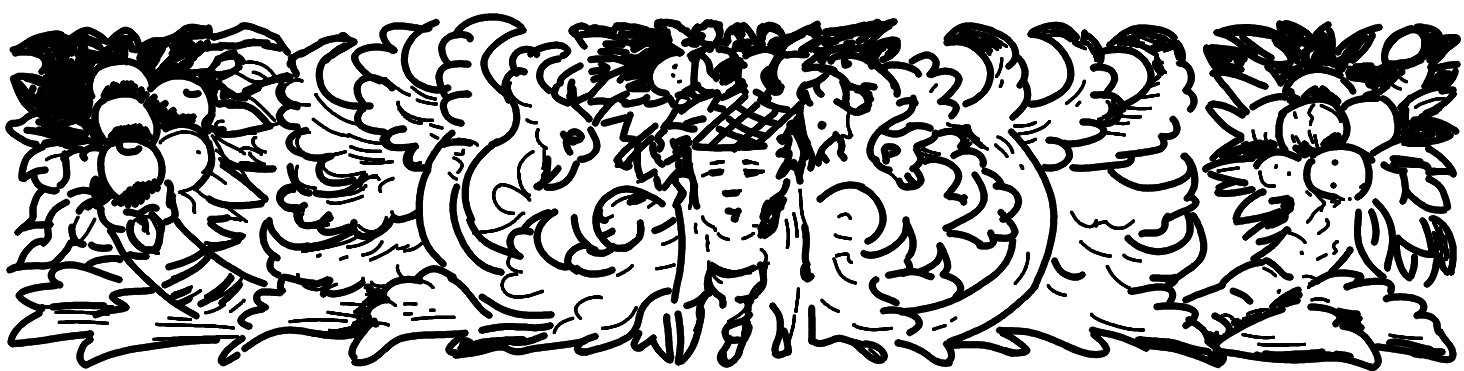
\includegraphics[scale=0.135]{images/en-tete-discours-sur-le-dessein.png}
	\bigbreak
	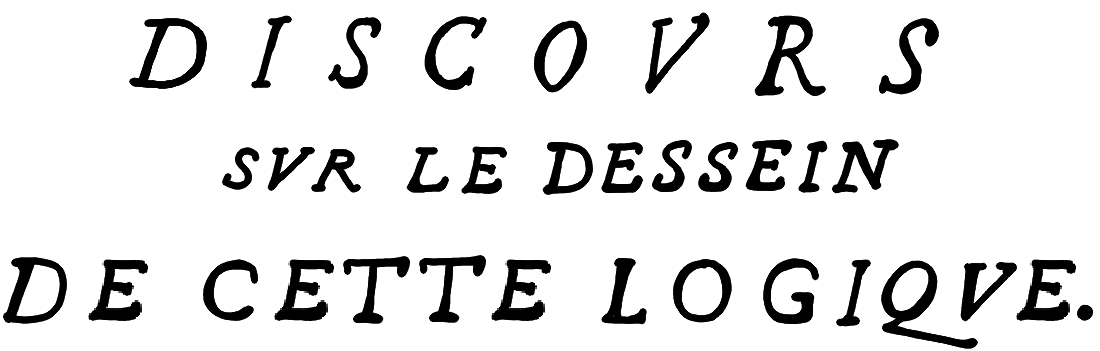
\includegraphics[scale=0.16]{images/titre-discours-sur-le-dessein.png}
\end{center}

\begin{wrapfigure}[5]{l}{0pt}
    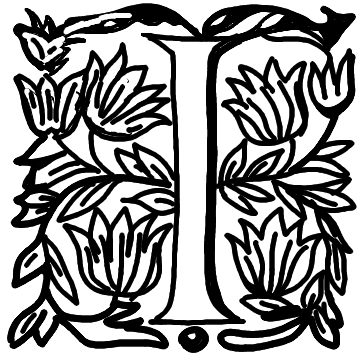
\includegraphics[width=0.25\textwidth]{images/enluminure-I.png}
\end{wrapfigure}
\noindent\hspace{13cm}{\texttt{L}} L n'y a rien de plus estimable que le bon sens et la justesse de l'esprit dans le discernement du vrai et du faux. Toutes les autres qualités d'esprit ont des usages bornés; mais l'exactitude de la raison est généralement utile dans toutes les parties et dans tous les emplois de la vie. Ce n'est pas seulement dans les sciences qu'il est difficile de distinguer la vérité de l'erreur ; mais aussi dans la plupart des sujets dont les hommes parlent, et des affaires qu'ils traitent. Il y a presque partout des routes différentes, les unes vraies, les autres fausses, et c'est à la raison d'en faire le choix. Ceux qui choisissent bien sont ceux qui ont l'esprit juste ; ceux qui prennent le mauvais parti sont ceux qui ont l'esprit faux ; et c'est la première et la plus importante différence qu'on peut mettre entre les qualités de l'esprit des hommes.

Ainsi, la principale application qu'on devrait avoir serait de former son jugement et de le rendre aussi exact qu'il le peut être ; et c'est à quoi devrait tendre la plus grande partie de nos études. On se sert de la raison comme d'un instrument pour acquérir les sciences, et l'on devrait se servir, au contraire, des sciences comme d'un instrument pour perfectionner sa raison ; la justesse de l'esprit étant infiniment plus considérable que toutes les connaissances spéculatives auxquelles on peut arriver par le moyen des sciences les plus véritables et les plus solides : ce qui doit porter les personnes sages à ne s'y engager qu'autant qu'elles peuvent servir à cette fin, et à n'en faire que l'essai et non l'emploi des forces de leur esprit.

Si l'on ne s'y applique dans ce dessein, on ne voit pas que l'étude de ces sciences spéculatives, comme de la géométrie, de l'astronomie et de la physique, soit autre chose qu'un amusement assez vain, ni qu'elles soient beaucoup plus estimables que l'ignorance de toutes ces choses, qui a au moins cet avantage, qu'elle est moins pénible, et qu'elle ne donne pas lieu à la sotte vanité que l'on tire souvent de ces connaissances stériles et infructueuses.

Non seulement ces sciences ont des recoins et des enfoncements fort peu utiles ; mais elles sont toutes inutiles, si on les considère en elles-mêmes et pour elles-mêmes. Les hommes ne sont pas nés pour employer leur temps à mesurer des lignes, à examiner les rapports des angles, à considérer les divers mouvements de la matière. Leur esprit est trop grand, leur vie trop courte, leur temps trop précieux pour l'occuper à de si petits objets ; mais ils sont obligés d'être justes, équitables, judicieux dans tous leurs discours, dans toutes leurs actions et dans toutes les affaires qu'ils manient, et c'est à quoi ils doivent particulièrement s'exercer et se former.

Ce soin et cette étude est d'autant plus nécessaire, qu'il est étrange combien c'est une qualité rare que cette exactitude de jugement. On ne rencontre partout que des esprits faux, qui n'ont presque aucun discernement de la vérité; qui prennent toutes choses d'un mauvais biais ; qui se payent des plus mauvaises raisons, et qui veulent en payer les autres ; qui se laissent emporter par les moindres apparences ; qui sont toujours dans l'excès et dans les extrémités ; qui n'ont point de serre pour se tenir fermes dans les vérités qu'ils savent, parce que c'est plutôt le hasard qui les y attache qu'une solide lumière ; ou qui s'arrêtent, au contraire, à leur sens avec tant d'opiniâtreté, qu'ils n'écoutent rien de ce qui pourrait les détromper ; qui décident hardiment ce qu'ils ignorent, ce qu'ils n'entendent pas, et ce que personne n'a peut-être jamais entendu ; qui ne font point de différence entre parler et parler, ou qui ne jugent de la vérité des choses que par le ton de la voix : celui qui parle facilement et gravement a raison ; celui qui a quelque peine à s'expliquer, ou qui fait paraître quelque chaleur, a tort. Ils n'en savent pas davantage.

C'est pourquoi il n'y a point d'absurdités si insupportables qui ne trouvent des approbateurs. Quiconque a dessein de piper le monde, est assuré de trouver des personnes qui seront bien aises d'être pipées ; et les plus ridicules sottises rencontrent toujours des esprits auxquels elles sont proportionnées, Après que l'on voit tant de gens infatués des folies de l'astrologie judiciaire, et que des personnes graves traitent cette matière sérieusement, on ne doit plus s'étonner de rien. Il y a une constellation dans le ciel qu'il a plu à quelques personnes de nommer Balance, et qui ressemble à une balance comme à un moulin à vent : la balance est le symbole de la justice : donc ceux qui naîtront sous cette constellation seront justes et équitables. Il y a trois autres signes dans le Zodiaque, qu'on nomme l'un Bélier, l'autre Taureau, l'autre Capricorne, et qu'on eût pu aussi bien appeler Éléphant, Crocodile et Rhinocéros : le bélier, le taureau et le capricorne sont des animaux qui ruminent ; donc ceux qui prennent médecine lorsque la lune est sous ces constellations, sont en danger de la revomir. Quelque extravagants que soient ces raisonnements, il se trouve des personnes qui les débitent, et d'autres qui s'en laissent persuader.

Cette fausseté d'esprit n'est pas seulement cause des erreurs que l'on mêle dans les sciences, mais aussi de la plupart des fautes que l'on commet dans la vie civile, des querelles injustes, des procès mal fondés, des avis téméraires, des entreprises mal concertées. Il y en a peu qui n'aient leur source dans quelque erreur et dans quelque faute de jugement : de sorte qu'il n'y a point de défaut dont on ait plus d'intérêt de se corriger.

Mais autant cette correction est souhaitable, autant est-il difficile d'y réussir, parce qu'elle dépend beaucoup de la mesure d'intelligence que nous apportons en naissant. Le sens commun n'est pas une qualité si commune que l'on pense. Il y a une infinité d'esprits grossiers et stupides que l'on ne peut réformer en leur donnant l'intelligence de la vérité, mais en les retenant dans les choses qui sont à leur portée, et en les empêchant de juger de ce qu'ils ne sont pas capables de connaître. Il est vrai néanmoins qu'une grande partie des faux jugements des hommes ne vient pas de ce principe, et qu'elle n'est causée que par la précipitation de l'esprit et par le défaut d'attention, qui fait que l'on juge témérairement de ce que l'on ne connaît que confusément et obscurément. Le peu d'amour que les hommes ont pour la vérité fait qu'ils ne se mettent pas en peine la plupart du temps de distinguer ce qui est vrai de ce qui est faux. Ils laissent entrer dans leur âme toutes sortes de discours et de maximes; ils aiment mieux les supposer pour véritables que de les examiner : s'ils ne les entendent pas, ils veulent croire que d'autres les entendent bien ; et ainsi ils se remplissent la mémoire d'une infinité de choses fausses, obscures et non entendues, et raisonnent ensuite sur ces principes, sans presque considérer ni ce qu'ils disent, ni ce qu'ils pensent.

La vanité et la présomption contribuent encore beaucoup à ce défaut. On croit qu'il y a de la honte à douter et à ignorer; et l'on aime mieux parler et décider au hasard que de reconnaître qu'on n'est pas assez informé des choses pour en porter jugement. Nous sommes tous pleins d'ignorance et d'erreurs ; et cependant on à toutes les peines du monde à tirer de la bouche des hommes cette confession si juste et si conforme à leur condition naturelle : je me trompe, et je n'en sais rien.

Il s'en trouve d'autres au contraire qui ayant assez de lumières pour connaître qu'il y a quantité de choses obscures et incertaines, et voulant, par une autre sorte de vanité, témoigner qu'ils ne se laissent pas aller à la crédulité populaire, mettent leur gloire à soutenir qu'il n'y a rien de certain : ils se déchargent ainsi de la peine de les examiner, et, sur ce mauvais principe, ils mettent en doute les vérités les plus constantes, et la Religion même. C'est la source du Pyrrhonisme, qui est une autre extravagance de l'esprit humain, qui, paraissant contraire à la témérité de ceux qui croient et décident tout, vient néanmoins de la même source, qui est le défaut d'attention ; car comme les uns ne veulent pas se donner la peine de discerner les erreurs, les autres ne veulent pas prendre celle d'envisager la vérité avec le soin nécessaire pour en apercevoir l'évidence. La moindre lueur suffit aux uns pour les persuader de choses très fausses, et elle suffit aux autres pour les faire douter des choses les plus certaines : mais, dans les uns et dans les autres, c'est le même défaut d'application qui produit des effets si différents.

La vraie raison place toutes choses dans le rang qui leur convient; elle fait douter de celles qui sont douteuses, rejeter celles qui sont fausses, et reconnaître de bonne foi celles qui sont évidentes, sans s'arrêter aux vaines raisons des Pyrrhoniens, qui ne détruisent pas l'assurance raisonnable que l'on a des choses certaines, non pas même dans l'esprit de ceux qui les proposent. Personne ne douta jamais sérieusement qu'il y a une terre, un soleil et une lune, ni si le tout est plus grand que sa partie. On peut bien faire dire extérieurement à sa bouche qu'on en doute, parce que l'on peut mentir ; mais on ne peut pas le faire dire à son esprit. Ainsi le Pyrrhonisme n'est pas une secte de gens qui soient persuadés de ce qu'ils disent, mais c'est une secte de menteurs. Aussi se contredisent-ils souvent en parlant de leur opinion, leur cœur ne pouvant s'accorder avec leur langue, comme on peut le voir dans Montaigne, qui a tâché de le renouveler au dernier siècle.

Car, après avoir dit que les Académiciens étaient différents des Pyrrhoniens, en ce que les Académiciens avouaient qu'il y avait des choses plus vraisemblables que les autres, ce que les Pyrrhoniens ne voulaient pas reconnaître, il se déclare pour les Pyrrhoniens en ces termes : \emph{L'avis}, dit-il, \emph{des Pyrrhoniens est plus hardi, et quant et quant plus vraisemblable}. Il y a donc des choses plus vraisemblables que les autres : et ce n'est pas pour faire une pointe qu'il parle ainsi; ce sont des paroles qui lui sont échappées sans y penser, et qui naissent du fond de la nature, que le mensonge des opinions ne peut étouffer.

Mais le mal est que, dans les choses qui ne sont pas si sensibles, ces personnes, qui mettent leur plaisir à douter de tout, empêchent leur esprit de s'appliquer à ce qui pourrait les persuader, ou ne s'y appliquent qu'imparfaitement, et ils tombent par là dans une incertitude volontaire à l'égard des choses de la Religion, parce que cet état de ténèbres qu'ils se procurent leur est agréable, et leur paraît commode pour apaiser les remords de leur conscience, et pour contenter librement leurs passions.

Ainsi, comme ces dérèglements d'esprit, qui paraissent opposés, l'un portant à croire légèrement ce qui est obscur et incertain, et l'autre à douter de ce qui est clair et certain, ont néanmoins le même principe, qui est la négligence à se rendre attentif autant qu'il faut pour discerner la vérité, il est visible qu'il faut y remédier de la même sorte, et que l'unique moyen de s'en garantir est d'apporter une attention exacte à nos jugements et à nos pensées. C'est la seule chose qui soit absolument nécessaire pour se défendre des surprises : car ce que les Académiciens disaient, qu'il était impossible de trouver la vérité, si on n'en avait des marques, comme on ne pourrait reconnaître un esclave fugitif qu'on chercherait si on n'avait des signes pour le distinguer des autres, au cas qu'on le rencontrât, n'est qu'une vaine subtilité. Comme il ne faut point d'autres marques pour distinguer la lumière des ténèbres, que la lumière même qui se fait sentir, ainsi, il n'en faut point d'autres pour reconnaître la vérité, que la clarté même qui l'environne, et qui se soumet l'esprit et le persuade malgré qu'il en ait; de sorte que toutes les raisons de ces philosophes ne sont pas plus capables d'empêcher l'âme de se rendre à la vérité, lorsqu'elle en est fortement pénétrée, qu'elles sont capables d'empêcher les yeux de voir, lorsqu'étant ouverts, ils sont frappés par la lumière du soleil,

Mais, parce que l'esprit se laisse quelquefois abuser par de fausses lueurs, lorsqu'il n'y apporte pas l'attention nécessaire, et qu'il y a bien des choses que l'on ne connaît que par un long et difficile examen, il est certain qu'il serait utile d'avoir des règles pour s'y conduire de telle sorte, que la recherche de la vérité en fût et plus facile et plus sûre ; et ces règles, sans doute, ne sont pas impossibles. Car, puisque les hommes se trompent quelquefois dans leurs jugements, et que, quelquefois aussi, ils ne se trompent pas, qu'ils raisonnent tantôt bien et tantôt mal, et qu'après avoir mal raisonné, ils sont capables de reconnaître leur faute, ils peuvent remarquer, en faisant des réflexions sur leurs pensées, quelle méthode ils ont suivie, lorsqu'ils ont bien raisonné, et quelle a été la cause de leur erreur, lorsqu'ils se sont trompés, et former ainsi des règles sur ces réflexions, pour éviter à l'avenir d'être surpris.

C'est proprement ce que les philosophes entreprennent, et sur quoi ils nous font des promesses magnifiques. Si on veut les en croire, ils nous fournissent, dans cette partie qu'ils destinent à cet effet, et qu'ils appellent Logique, une lumière capable de dissiper toutes les ténèbres de notre esprit ; ils corrigent toutes les erreurs de nos pensées, et ils nous donnent des règles si sûres, qu'elles nous conduisent infailliblement à la vérité, et si nécessaires tout ensemble, que, sans elles, il est impossible de la connaître avec une entière certitude. Ce sont les éloges qu'ils donnent eux-mêmes à leurs préceptes. Mais, si l'on considère ce que l'expérience nous fait voir de l'usage que ces philosophes en font, et dans la logique, et dans les autres parties de la philosophie, on aura beaucoup de sujet de se défier de la vérité de ces promesses.

Néanmoins, parce qu'il n'est pas juste de rejeter absolument ce qu'il y a de bon dans la logique, à cause de l'abus qu'on peut en faire, et qu'il n'est pas vraisemblable que tant de grands esprits, qui se sont appliqués avec tant de soin aux règles du raisonnement, n'aient rien du tout trouvé de solide ; et enfin parce que la coutume a introduit une certaine nécessité de savoir au moins grossièrement ce que c'est que logique, on a cru que ce serait contribuer en quelque chose à l'utilité publique, que d'en tirer ce qui peut le plus servir à former le jugement. Et c'est proprement le dessein qu'on s'est proposé dans cet ouvrage, en y ajoutant plusieurs nouvelles réflexions qui sont venues dans l'esprit en écrivant, et qui en font la plus grande et peut-être la plus considérable partie.

Car il semble que les philosophes ordinaires ne se soient guère appliqués qu'à donner des règles des bons et des mauvais raisonnements. Or, quoique l'on ne puisse pas dire que ces règles soient inutiles, puisqu'elles servent quelquefois à découvrir le défaut de certains arguments embarrassés, et à disposer ses pensées d'une manière plus convaincante, néanmoins on ne doit pas aussi croire que cette utilité s'étende bien loin, la plupart des erreurs des hommes ne consistant pas à se laisser tromper par de mauvaises conséquences, mais à se laisser aller à de faux jugements dont on tire de mauvaises conséquences. C'est à quoi ceux qui jusqu'ici ont traité de la Logique ont peu cherché de remèdes, et ce qui fait le principal sujet des nouvelles réflexions qu'on trouvera partout dans ce livre.

On est obligé néanmoins de reconnaître que ces réflexions, qu'on appelle nouvelles, parce qu'on ne les voit pas dans les Logiques communes, ne sont pas toutes de celui qui a travaillé à cet ouvrage, et qu'il en a emprunté quelques-unes des livres d'un célèbre philosophe de ce siècle, qui a autant de netteté d'esprit qu'on trouve de confusion dans les autres. On en a aussi tiré quelques autres d'un petit écrit non imprimé, qui avait été fait par feu M. Pascal, et qu'il avait intitulé, \emph{De l'esprit géométrique}, et c'est ce qui est dit dans le Chapitre IX de la première partie, de la différence des définitions de noms et des définitions de choses, et les cinq règles qui sont expliquées dans la quatrième partie, que l'on y a beaucoup plus étendues qu'elles ne le sont dans cet écrit.

Quant à ce qu'on a tiré des livres ordinaires de la logique, voici ce qu'on y a observé :

Premièrement, on a eu dessein de renfermer dans celle-ci tout ce qui était véritablement utile dans les autres, comme les règles des figures, les divisions des termes et des idées, quelques réflexions sur les propositions. Il y avait d'autres choses qu'on jugeait assez inutiles, comme les catégories et les lieux; mais parce qu'elles étaient courtes, faciles et communes, on n'a pas cru devoir les omettre, en avertissant néanmoins du jugement qu'on doit en faire, afin qu'on ne les crût pas plus utiles qu'elles ne sont.

On a été plus en doute sur certaines matières assez épineuses et peu utiles, comme les conversions des propositions, la démonstration des règles des figures, mais enfin on s'est résolu de ne pas les retrancher, la difficulté même n'en étant pas entièrement inutile. Car il est vrai que, lorsqu'elle ne se termine à la connaissance d'aucune vérité, on a raison de dire : \emph{Stultum est difficiles habere nugas} : mais on ne doit pas l'éviter de même, quand elle mène à quelque chose de vrai, parce qu'il est avantageux de s'exercer à entendre les vérités difficiles.

Il y a des estomacs qui ne peuvent digérer que les viandes légères et délicates ; et il y a de même des esprits qui ne peuvent s'appliquer à comprendre que les vérités faciles et revêtues des ornements de l'éloquence. L'un et l'autre est une délicatesse blâmable, ou plutôt une véritable faiblesse. Il faut rendre son esprit capable de découvrir la vérité, lors même qu'elle est cachée et enveloppée, et de la respecter sous quelque forme qu'elle paraisse. Si on ne surmonte cet éloignement et ce dégoût, qu'il est facile à tout le monde de concevoir de toutes les choses qui paraissent un peu subtiles et scolastiques, on étrécit insensiblement son esprit, et on le rend incapable de comprendre ce qui ne se connaît que par l'enchaînement de plusieurs propositions : et, ainsi, quand une vérité dépend de trois ou quatre principes qu'il est nécessaire d'envisager tout à la fois, on s'éblouit, on se rebute, et l'on se prive par ce moyen de la connaissance de plusieurs choses utiles ; ce qui est un défaut considérable.

La capacité de l'esprit s'étend et se resserre par l'accoutumance, et c'est à quoi servent principalement les mathématiques, et généralement toutes les choses difficiles, comme celles dont nous parlons; car elles donnent une certaine étendue à l'esprit, et elles l'exercent à s'appliquer davantage et à se tenir plus ferme dans ce qu'il connaît.

Ce sont les raisons qui ont porté à ne pas omettre ces matières épineuses, et à les traiter même aussi subtilement qu'en aucune autre Logique. Ceux qui n'en seront pas satisfaits peuvent s'en délivrer en ne les lisant pas ; car on a eu soin pour cela de les en avertir à la tête même des chapitres, afin qu'ils n'aient pas sujet de s'en plaindre, et que s'ils les lisent, ce soit volontairement.

On n'a pas cru aussi devoir s'arrêter au dégoût de quelques personnes qui ont en horreur certains termes artificiels qu'on a formés pour retenir plus facilement les diverses manières de raisonner, comme si c'étaient des mots de magie, et qui font souvent des railleries assez froides sur \emph{baroco} et \emph{baralepton}, comme tenant du caractère de pédant ; parce que l'on à jugé qu'il y avait plus de bassesse dans ces railleries que dans ces mots. La vraie raison et le bon sens ne permettent pas qu'on traite de ridicule ce qui ne l'est point. Or, il n'y a rien de ridicule dans ces termes, pourvu qu'on n'en fasse pas un trop grand mystère ; et que, comme ils n'ont été faits que pour soulager la mémoire, on ne veuille pas les faire passer dans l'usage ordinaire, et dire, par exemple, qu'on va faire un argument en \emph{bocardo} ou en \emph{felapton}, ce qui serait en effet très ridicule.

On abuse quelquefois beaucoup de ce reproche de pédanterie, et souvent on y tombe en l'attribuant aux autres. La pédanterie est un vice d'esprit et non de profession ; et il y a des pédants de toutes robes, de toutes conditions et de tous états. Relever des choses basses et petites, faire une vaine montre de sa science, entasser du grec et du latin sans jugement, s'échauffer sur l'ordre des mois attiques, sur les habits des Macédoniens et sur de semblables disputes de nul usage ; piller un auteur en lui disant des injures, déchirer outrageusement ceux qui ne sont pas de notre sentiment sur l'intelligence d'un passage de Suetone, ou sur l'étymologie d'un mot, comme s'il s'y agissait de la religion et de l'État: vouloir faire soulever tout le monde contre un homme qui n'estime pas assez Cicéron, comme contre un perturbateur du repos public, ainsi que Jules Scaliger a tâché de faire contre Erasme, s'intéresser pour la réputation d'un ancien philosophe, comme si l'on était son proche parent, c'est proprement ce qu'on peut appeler pédanterie ; mais il n'y en a point à entendre ni à expliquer des mots artificiels assez ingénieusement inventés, et qui n'ont pour but que le soulagement de la mémoire, pourvu qu'on en use avec les précautions que l'on a marquées.

Il ne reste plus qu'à rendre raison pourquoi on a omis grand nombre de questions qu'on trouve dans les Logiques ordinaires, comme celles qu'on traite dans les prolégomènes, l'universel \emph{a parte rei}, les relations et plusieurs autres semblables ; et sur cela il suffirait presque de répondre qu'elles appartiennent plutôt à la métaphysique qu'à la logique. Mais il est vrai néanmoins que ce n'est pas ce qu'on a principalement considéré ; car quand on a jugé qu'une matière pouvait être utile pour former le jugement, on a peu regardé à quelle science elle appartenait. L'arrangement de nos diverses connaissances est libre comme celui des lettres d'une imprimerie; chacun a droit d'en former différents ordres, selon son besoin, quoique, lorsqu'on en forme, on les doive ranger de la manière la plus naturelle : il suffit qu'une matière nous soit utile pour nous en servir, et la regarder non comme étrangère, mais comme propre. C'est pourquoi on trouvera ici quantité de choses de physique et de morale, et presque autant de métaphysique qu'il est nécessaire d'en savoir, quoique l'on ne prétende point pour cela avoir emprunté rien de personne. Tout ce qui sert à la Logique lui appartient ; et c'est une chose entièrement ridicule que les gênes que se donnent certains auteurs, comme Ramus et les Ramistes, quoique d'ailleurs fort habiles gens, qui prennent autant de peine pour borner les juridictions de chaque science, et faire qu'elles n'entreprennent pas les unes sur les autres, que l'on en prend pour marquer les limites des royaumes et régler les ressorts des parlements.

Ce qui a porté aussi à retrancher entièrement ces questions d'école, n'est pas simplement de ce qu'elles sont difficiles et de peu d'usage : on en a traité quelques-unes de cette nature; mais c'est qu'ayant toutes ces mauvaises qualités, on a cru de plus qu'on pourrait se dispenser d'en parler sans choquer personne, parce qu'elles sont peu estimées.

Car il faut mettre une grande différence entre les questions inutiles dont les livres de philosophie sont remplis. Il y en a qui sont assez méprisées par ceux mêmes qui les traitent, et il y en à, au contraire, qui sont célèbres et autorisées, et qui ont beaucoup de cours dans les écrits de personnes d'ailleurs estimables.

Il semble que c'est un devoir auquel on est obligé à l'égard de ces opinions communes et célèbres, quelque fausses qu'on les croie, de ne pas ignorer ce qu'on en dit. On doit cette civilité, ou plutôt cette justice, non à la fausseté, car elle n'en mérite point, mais aux hommes qui en sont prévenus, de ne pas rejeter ce qu'ils estiment sans l'examiner. Et ainsi il est raisonnable d'acheter, par la peine d'apprendre ces questions, le droit de les mépriser.

Mais on a plus de liberté dans les premières ; et celles de logique, que nous avons cru devoir omettre, sont de ce genre : elles ont cela de commode qu'elles ont peu de crédit, non seulement dans le monde où elles sont inconnues, mais parmi ceux-là même qui les enseignent. Personne, Dieu merci, ne prend intérêt à l'universel \emph{a parte rei}, à l'être de raison, ni aux secondes intentions ; et ainsi on n'a pas lieu d'appréhender que quelqu'un se choque de ce qu'on n'en parle point ; outre que ces matières sont si peu propres à être mises en français, qu'elles auraient été plus capables de décrier la philosophie de l'École, que de la faire estimer.

Il est bon aussi d'avertir qu'on s'est dispensé de suivre toujours les règles d'une méthode tout à fait exacte, ayant mis beaucoup de choses dans la quatrième partie qu'on aurait pu rapporter à la seconde et à la troisième; mais on l'a fait à dessein, parce qu'on a jugé qu'il était utile de voir en un même lieu tout ce qui était nécessaire pour rendre une science parfaite ; ce qui est le plus grand ouvrage de la méthode dont on traite dans la quatrième partie : et c'est pour cette raison qu'on a réservé de parler en ce lieu-là des axiomes et des démonstrations.

Voilà à peu près les vues que l'on a eues dans cette Logique. Peut-être qu'avec tout cela il y aura fort peu de personnes qui en profitent, ou qui s'aperçoivent du fruit qu'elles en tireront ; parce qu'on ne s'applique guère d'ordinaire à mettre en usage des préceptes par des réflexions expresses ; mais on espère néanmoins que ceux qui l'auront lue avec quelque soin pourront en prendre une teinture qui les rendra plus exacts et plus solides dans leurs jugements, sans même qu'ils y pensent, comme il y a de certains remèdes qui guérissent des maux, en augmentant la vigueur et en fortifiant les parties. Quoi qu'il en soit, au moins n'incommodera-t-elle pas longtemps personne, ceux qui sont un peu avancés pouvant la lire et apprendre en sept ou huit jours ; et il est difficile que, contenant une si grande diversité de choses, chacun n'y trouve de quoi se payer de la peine de sa lecture.
